\documentclass[11pt,twocolumn]{article} % letterpaper is american!
\usepackage[affil-it]{authblk}

\usepackage[USenglish,american]{babel}
\usepackage[pdftex]{graphicx}
\usepackage{epstopdf}

\usepackage{cite}

\usepackage{amsfonts,amsmath,amsthm,amssymb}

\usepackage{tikz,pgf}
\usetikzlibrary{fit}

\usepackage{csvsimple}

%\pagestyle{empty}
\setlength{\parindent}{0mm}
\usepackage[letterpaper, margin=1in]{geometry}
%\usepackage{showframe}

\usepackage{multicol}
\usepackage{enumerate}

\usepackage{verbatim}
\usepackage{listings}

\usepackage{color}

%%
%% Julia definition (c) 2014 Jubobs
%%
\lstdefinelanguage{Julia}%
  {morekeywords={abstract,break,case,catch,const,continue,do,else,elseif,%
      end,export,false,for,function,immutable,import,importall,if,in,%
      macro,module,otherwise,quote,return,switch,true,try,type,typealias,%
      using,while},%
   sensitive=true,%
   alsoother={$},%
   morecomment=[l]\#,%
   morecomment=[n]{\#=}{=\#},%
   morestring=[s]{"}{"},%
   morestring=[m]{'}{'},%
}[keywords,comments,strings]%

\lstset{%
    language         = Python,
    basicstyle       = \footnotesize\ttfamily,,
    keywordstyle     = \bfseries\color{blue},
    stringstyle      = \color{magenta},
    commentstyle     = \color{red},
    showstringspaces = false,
    backgroundcolor  = \color{lightgray},
    numbers          = left,
    title            = \lstname,
    numberstyle      = \tiny\color{lightgray}\ttfamily,
}

\usepackage{xspace}
\usepackage{url}
\usepackage{cite}

\usepackage{coffee4}

\usepackage{titlesec}
\titlespacing*{\subsubsection}{0pt}{*0}{*0}
\titlespacing*{\subsection}{0pt}{0pt}{*0}
\titlespacing*{\section}{0pt}{0pt}{*0}

\newcommand{\Bold}{\mathbf}

\setlength{\parskip}{1em}
%\setlength{\parindent}{1em}

\def\roi{region of interest\xspace}
\def\rois{regions of interest\xspace}
\def\tois{territory of interest\xspace}

\def\r{\texttt{red}\xspace}
\def\g{\texttt{green}\xspace}
\def\b{\texttt{blue}\xspace}

\def\cw{C\&W Energy Energy Solutions\xspace}
\def\rgb{RGB Optics\xspace}

\def\ida{International Darksky Administration\xspace}

\def\python{\texttt{python}\xspace}
\def\np{\texttt{numpy}\xspace}
\def\ndimage{\texttt{ndimage}\xspace}

\title{Remote Sensing Light Pollution with Pedestrian Equiptment}
\date{\today}
\author{Philip Robinson}
\affil{Oregon Health Sciences University}

\begin{document}

\twocolumn[\begin{@twocolumnfalse}

\maketitle

\begin{abstract}
  To think of light pollution as only impeding human's view of the night sky, ignores the impact of different light on non-human sensor systems. Many species of animal have involuntary Phototaxis~\cite{longcore,bridge} reactions to specific spectral ranges, which can result in significant consequences on the ecology of a region (especially in the case of migratory~\cite{salmon}, infant, and endangered species~\cite{turtle}). Likewise, high precision artificial sensor systems, like terrestrial telescopes and night vision scopes, are designed to perform best for their location's natural limitations; and may loose accuracy and precision when exposed to such light pollution.
  Unfortunately, the cost of auditing a cities impact on such systems usually requires testing light sources with expensive lab equipment; additionally, such approaches don't appreciate the exaggeration of effects caused by reflective surfaces in the environment and the shape of fixtures. There is interest in developing low cost audit tools for light-dense regions.
  We propose segmenting \rois from a cityscape, primarily driven by morphological watersheding, as the first step in this analysis. This approach yields intuitive \rois that clearly identify light sources and reflectors without the need of seeding. In addition, we propose some base metric strategies to introduce rigor to the field.
\end{abstract}

\end{@twocolumnfalse}]

\section{Introduction}
Light pollution is much more complicated than its traditional interpretation, as perceived by human eyes. More completely, light pollution describes a relationship between a light source and sensors being actuated within that sources reach. Many species of animal have involuntary Phototaxis~\cite{longcore,bridge} reactions to specific spectral ranges, which can result in significant consequences on the ecology of a region (especially in the case of migratory~\cite{salmon}, infant, and endangered species~\cite{turtle}). Likewise, high precision artificial sensor systems, like terrestrial telescopes and night vision scopes, are designed to perform best for their location's natural limitations; and may loose accuracy and precision when exposed to certain types of light pollution.

There is interest in identifying a low cost means to audit and measure the light pollution (as captured in a cityscapes). Ideally, the use of low cost hardware, would allow citizens and interested parties to better understand light profile relationships to known native sensor systems. Additionally, as certain lighting technologies become obsolete and too expensive to maintain, like the low pressure sodium bulbs formerly found in Waimea HI, such technology can be used to inform municipalities of the consequences of their lighting decisions on native sensor systems.

In studying light pollution, from photographs, there are clear challenges needing to be addressed. The first is identifying light emitting sources from our images. Second is growing separate regions, large enough to provide useful summary statistics on their sources, that don't include multiple sources. Third is to establish summary statistics that are useful in defining simplified light profiles for each region.

The idiom ``pooling light'' intuitively describes how light is emitted about it's environment, and leads us to consider morphological watersheding as a segmentation and region growing technique. Morphological watersheding treats an image like a topological map and successively grows region pools by simulating water's behavior on that map. Using inverse light intensity as elevation in this algorithm is a natural fit for both source identification and segmentation. %Establishing summary statistics will be future work.

Other segmentation strategies can be used to identify \rois in an image, however morphological watersheds allow a segment to include the largest natural region containing a single light source (or reflective surface) as its major contributing pollutant. Once the original segments have been established, later processing (including subsetting) may be done to regions in order to generate useful summary statistics. As an added strength to this approach, morphological watersheding doesn't require seeding it's regions (reducing the number of hyper-parameters).

Simple Voronoi tessellation, divides regions without taking into account differences in intensities between multiple sources. These intensity deltas may be consequence of general intensity of individual sources, which is expected to be informative. Segmentation by random walks, other than being non-deterministic, asks all random walkers take a similar number of steps. This disproportionately weights high intensity local minima, like those found to be reflectors rather than light sources. Both of these strategies require seeding.

\section{Prior Work}
Much of the prior work in this space comes from different disciplines, with varying levels of rigor. Additionally, data collectors haven't agreed on what to measure. Nightglow~\cite{ida} is the metric of the \ida, which is measured by trained humans through self reporting star visibility. Similar ambient light metrics are used with low cost cameras~\cite{camera}, but unfortunately doesn't yield information about the individual light sources and can be easily biased by natural effects (like moonlight and scattering caused by clouds).

\section{Methods}

\subsection{Morphological Watershed}
The segmentation approach implemented is morphological watersheding~\cite{dip}. Morphological watersheding builds catchment pools by taking iterative slices of an image parallel to the intensity plane, in order to grow existing regions that contain local minima as created by that slice or below. This algorithm is simply visualized in \texttt{(Figure~\ref{fig:demo})}.

\begin{figure}
  \begin{multicols}{3}
    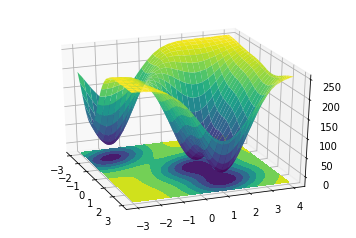
\includegraphics[width=\columnwidth]{./images/algorithm/generated.png}

    
\includegraphics[width=\columnwidth]{./images/algorithm/test_img.png}

    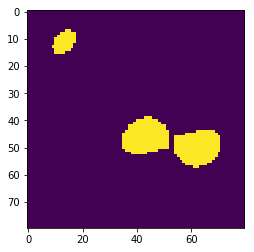
\includegraphics[width=\columnwidth]{./images/algorithm/split.png}
  \end{multicols}
        \caption{Watershed Algorithm}
        \label{fig:demo}
\end{figure}

For this algorithm, a gray scale image $\mathcal{G}$ acts as a topological map.
\[\mathbb{T}_\mathcal{G}(n) = \{(x,y) : \mathcal{G}(x,y) < n\}\]
defines the collection of points whose value is less than our water elevation level $n\in[0,255]$.
Let $\mathbb{C}(n-1)$ define set of catchments generated at elevation level $(n-1)$.
$\mathbb{Q}_\mathcal{G}(n)$ is the set of disconnected regions in $\mathbb{T}_\mathcal{G}(n)$.
For every region $q \in \mathbb{Q}_\mathcal{G}(n)$ three cases must be covered.

\[K_q = \big\vert\{c : c\cap q \neq \varnothing\}\big\vert\]
\begin{align*}
  K_q = 0  &\rightarrow\texttt{create new catchment}\\
  K_q = 1  &\rightarrow\texttt{merge region and catchment}\\
  \texttt{else}  &\rightarrow\texttt{grow catchments and build dams}
\end{align*}

The first two cases are trivial. The third is handled by performing dilation on the overlapping catchments from the prior elevation level, with a $3x3$ kernel, until $q$ is completely filled. Whenever growing catchments overlap, $\mathcal{G}$ is set to $255$ and those values act as damns preventing further growth. This is demonstrated in \texttt{(Figure~\ref{fig:regions})} ~\cite{dip}.

\begin{figure}
  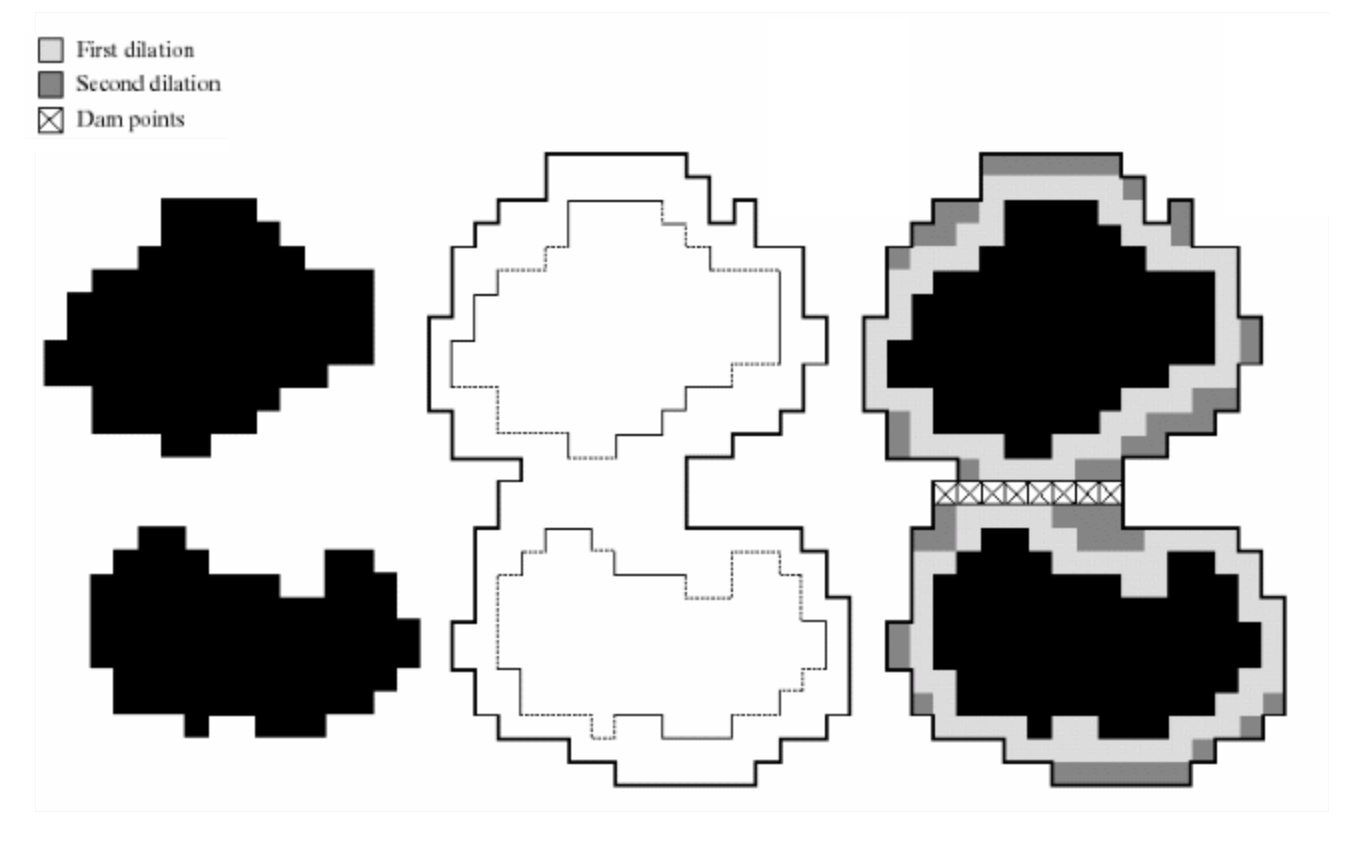
\includegraphics[width=\columnwidth]{./images/algorithm/regions.png}
  \caption{Region Growing}
  \label{fig:regions}
\end{figure}

Usually, because segmentation is driven by edge detection, morphological watersheding is performed on the derivative of an image, rather than it's raw values. In this case, the goal is to capture regions of diffuse light, which is modeled directly as pools by inverting the intensity values of a grayscale image. This has the effect of assigning high intensity regions to distinct pools.

\subsection{Implementation Details}
The algorithm was implemented in \python using \np and \ndimage for their array and image abstractions respectively. The catchments ledger is preserved (as a function of elevation level), so segmentation process may be animated.

This process is not completely automatic, as you must denoise the image in preprocessing. Since the approach focuses on catchments over diffuse light, and not edge detection, blurring does this job very easily. For any class of photo, the user is encouraged to select a gaussian blur filter of appropriate size for their image. This blurring model should also squash the star patterns in the image that are naturally looking artifacts of the camera, not a consequence of the environment.

The main hyperparameter to tune is $\sigma$ for the blur filter. Selecting too great a blur filter will join unique light sources like in \texttt{(Figure~\ref{fig:shared})}. Too small a filter will result in unjustifiable island regions, or regions defined by star patterns like in \texttt{(Figure~\ref{fig:star})}.

\begin{figure}
  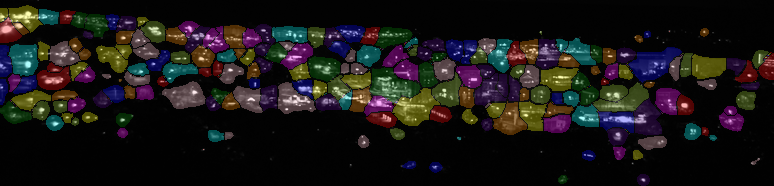
\includegraphics[width=\columnwidth]{./images/flagstaff-colored-160.png}
        \caption{Flagstaff - Shared Region}
        \label{fig:shared}
\end{figure}

\begin{figure}
  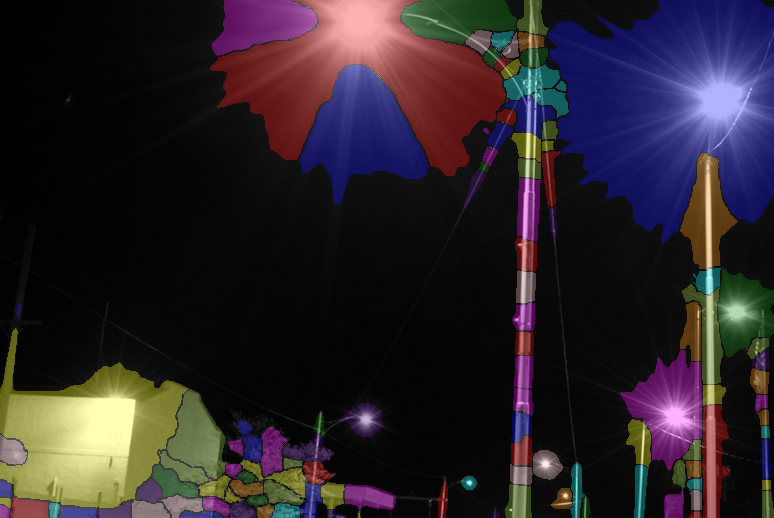
\includegraphics[width=\columnwidth]{./images/star.png}
        \caption{Winslow AZ - Star Region}
        \label{fig:star}
\end{figure}

In large files, there is often used a threshold, in order to satisfy computation time restraints. \texttt{(Figure~\ref{fig:wiama-colored})} contains a segmentation of Waimea HI, ignoring all intensity values less than 95/255, with a blurring filter of $(\sigma=3)$. That this segments nearly perfectly, with perhaps some room for better blurring (high resolution images are included in report submission).

\begin{figure}
  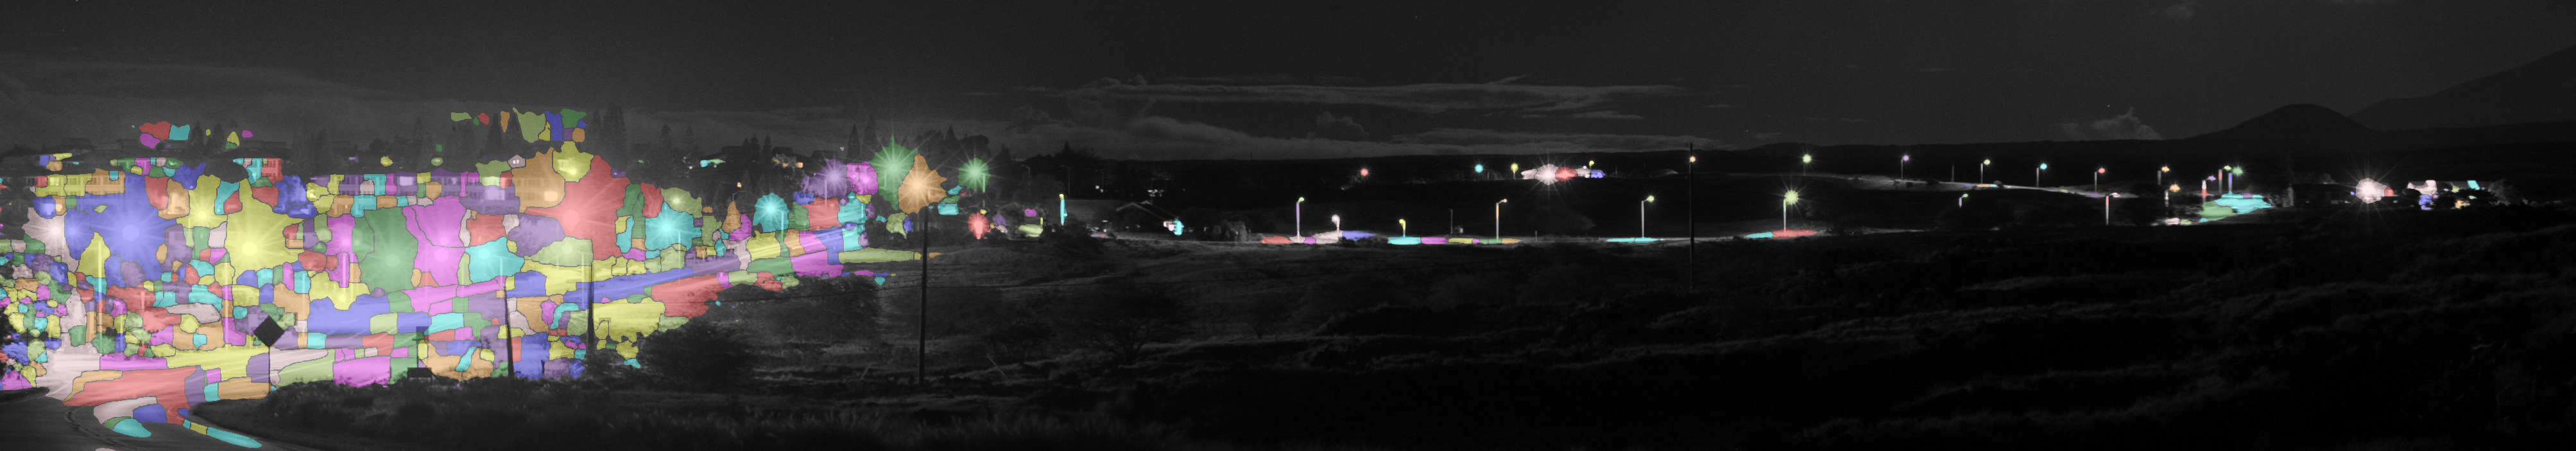
\includegraphics[width=\columnwidth]{./images/wiama-colored-160.png}
  \caption{Waimea HI - colored w/ threshold}
  \label{fig:wiama-colored}
\end{figure}

\section{Materials}

The raw data from this work came from a collaboration with \cw and \rgb. There is a collection of cityscapes of Waima HI, under the Mauna Kea Observatories \texttt{(Figure~\ref{fig:wiama})}
, and Flagstaff AZ,  under the Lowell Observatory \texttt{(Figure~\ref{fig:flagstaff})}. Along with photographs of specific street lamps and rows of street lamps that were installed for photographing in Winslow, AZ. For each picture the model of the camera, time, and location, are known and for the Winslow photographs the model of each installed street lamp is known as well \texttt{(Figure~\ref{fig:winslow})}.

\begin{figure}
        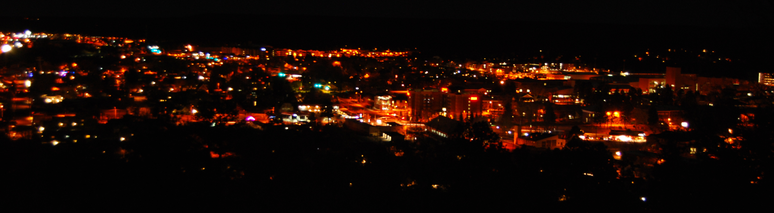
\includegraphics[width=\columnwidth]{./images/flagstaff.png}
        \caption{Flagstaff AZ}
        \label{fig:flagstaff}
\end{figure}

\begin{figure}
        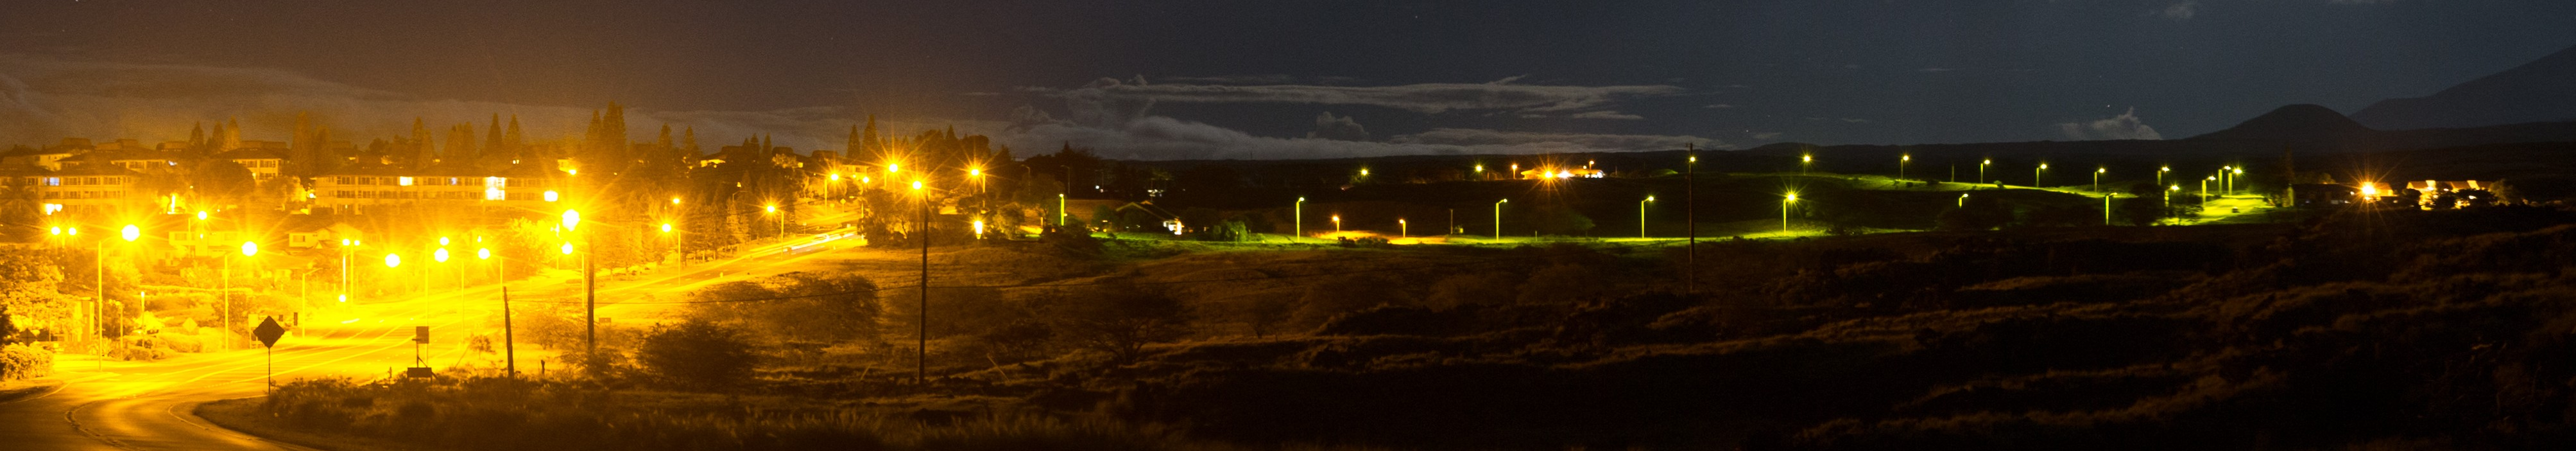
\includegraphics[width=\columnwidth]{./images/wiama.png}
        \caption{Waimea HI}
        \label{fig:wiama}
\end{figure}

\begin{figure}
  \begin{multicols}{3}
    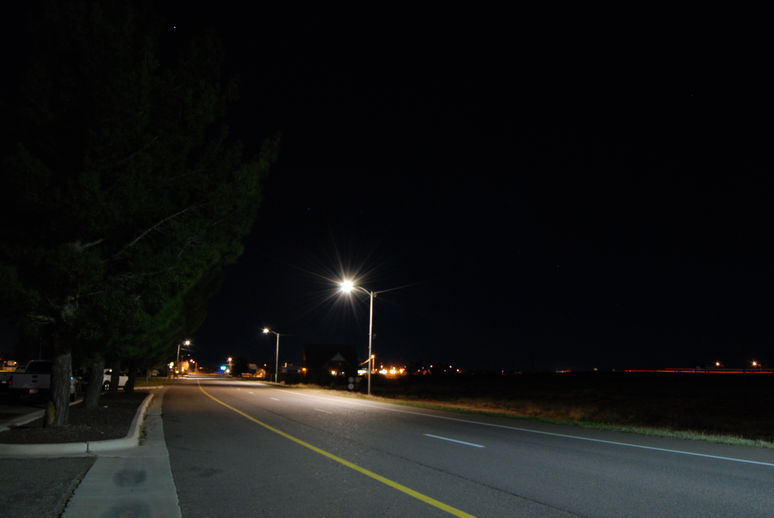
\includegraphics[width=\columnwidth]{./images/wa.png}

    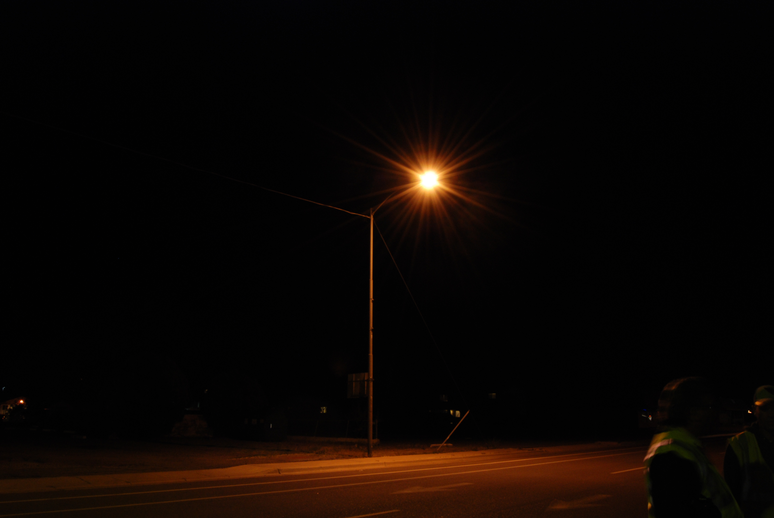
\includegraphics[width=\columnwidth]{./images/wb.png}

    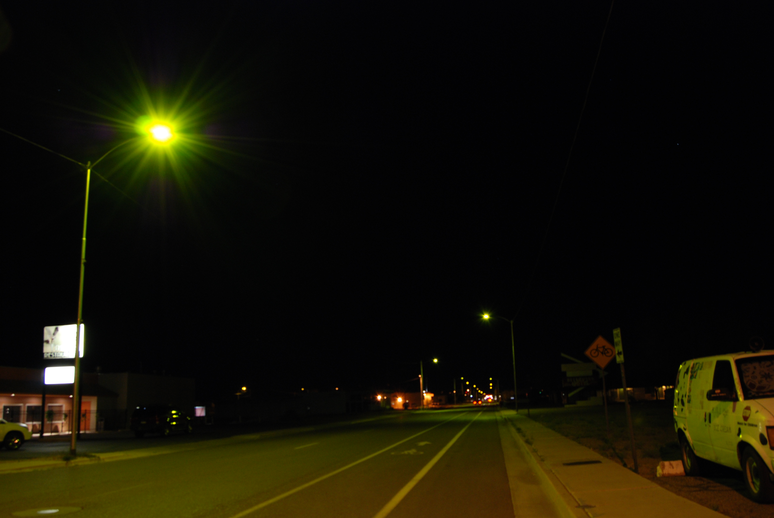
\includegraphics[width=\columnwidth]{./images/wc.png}
  \end{multicols}
        \caption{Winslow AZ}
        \label{fig:winslow}
\end{figure}

\section{Results}

For a closer look on how this approach performs against traditional segmentation competitors, \texttt{(Figure~\ref{fig:random})} generates an image more similar to Voronoi tessellation than an organic division. Random walkers also require seed points, which means the user must tune for identifying local minima in addition to the blurring filters. With more hyper parameters there is more complexity for the user, which pushes us further away from complete automation.

Additionally, the random walker will find resistance proportional to the steepness of neighboring intensity deltas, which disproportionately grows high valued local minima and restricts low valued local minima. You can see this in the growing size around reflective surfaces, and smaller size of the lamp housing regions.

\begin{figure}
  \begin{multicols}{3}
    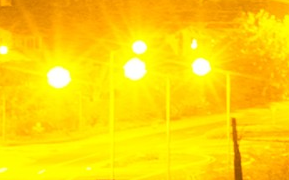
\includegraphics[width=\columnwidth]{./images/comparison/source.png}

    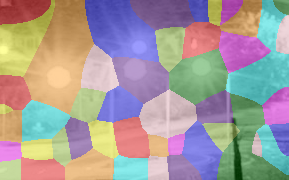
\includegraphics[width=\columnwidth]{./images/comparison/random.png}

    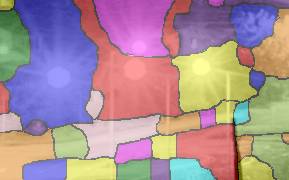
\includegraphics[width=\columnwidth]{./images/comparison/watershed.png}
  \end{multicols}
        \caption{Source vs Random Walk vs Watershed}
        \label{fig:random}
\end{figure}

\section{Discussion}

\subsection{Study Assumptions}
Pedestrian cameras attempt to approximate the behavior of a human eye, by measuring the activation of silicone sensors behind \r, \g, and \b filters in an area of the camera's sensor array. As a result, electromagnetic contributions specifically outside of the human color acuity range are not possible to capture. Luckily convergent evolution, driven by the atmosphere limiting the light that strikes earth, has resulted in many organic sensors to overlap in color acuity.

Camera manufacturers may also have proprietary transformations applied to make the images more aesthetically appealing. It is assumed that, because camera manufactures have a photo-realistic goal, that these proprietary modifications will have a negligible effect on the scale.

In order to prove this approach, gray-scaling the images happened before segmentation. It is understood that this approach may loose critical information for light sources that are heavily biased to one channel. Approaches to address this are discussed later in the paper.

Finally, saturated\footnote{a saturated sensor is one that is reporting the maximum possible value for that sensor} sensors may be used to help identify seeds for \rois, but become non-informative regions after segmentation. Although no further analytics in this paper, this is critical to know for future work.

\subsection{Data Acquisition}



\section{Next Steps}
The next big task will be to attempt to approximate the spectral profile of the light sources, or conversely attempt to automatically identify the type of bulb in an image. The later is acceptable, as the spectral profile of a bulb can be measured in a lab, then associate it with the image data. This however puts a heavier expense burden on the work. Identifying summary statistics and processing strategies for these regions is an open research question.

Finally, there are some cases, like reflections from clouds, where boundaries are non-informative. In these cases it would be valuable to explore generic segment joining algorithms. You can see this in \texttt{(Figure~\ref{fig:clouds})}. A robust agglomeration strategy to address this and similar concerns needs to be established.

\begin{figure}
  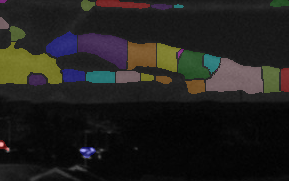
\includegraphics[width=\columnwidth]{./images/clouds.png}
  \caption{Waimea HI - clouds}
  \label{fig:clouds}
\end{figure}

\bibliography{references.bib}{}
\bibliographystyle{plain}


\end{document}
